\documentclass[10pt,article]{article}
\newcommand{\myMargin}{0.15in}
\usepackage[a4paper, margin=\myMargin]{geometry}
\usepackage{graphicx}
\usepackage{booktabs}
\usepackage{url}
\usepackage{enumitem}
\usepackage{palatino}
\usepackage{tabularx}
\usepackage{multicol}
\usepackage{xcolor}
\usepackage{enumitem}
\usepackage[hidelinks]{hyperref}
\fontfamily{SansSerif}
\usepackage{multirow}
% \usepackage{fontspec}
\usepackage{fontawesome}
% \usepackage[T1]{fontenc}

\selectfont

\usepackage[T1]{fontenc}
\usepackage
%[ansinew]
[utf8]
{inputenc}

\usepackage{color}
% \definecolor{myblue}{gray}{0.82}
\definecolor{myblue}{HTML}{96bfeb}
\definecolor{myred}{HTML}{961212}
\definecolor{nptel}{HTML}{c71254}
\textheight=10.75in
\raggedbottom

\setlength{\tabcolsep}{0in}
\newcommand{\isep}{-2 pt}
\newcommand{\lsep}{-0.5cm}
\newcommand{\psep}{-0.6cm}
\renewcommand{\labelitemii}{$\circ$}

\pagestyle{empty}
%-----------------------------------------------------------
%Custom commands
\newcommand{\resitem}[1]{\item #1 \vspace{-2pt}}
% \newcommand{\resheading}[1]{{\small \colorbox{myblue} { \begin{minipage}{0.99\textwidth}\centering{\textbf{#1 \vphantom{p\^{E}}}}\end{minipage}}}}
% \newcommand{\ressubheading}[3]{
% \begin{tabular*}{6.62in}{l @{\extracolsep{\fill}} r}
% 	\textsc{{\textbf{#1}}} & \rightline\textsc{\textit{[#2]}} \\
% \end{tabular*}\vspace{-8pt}}

\newcommand{\resheading}[1]{{\small \colorbox{myblue} { \begin{minipage}{\dimexpr\linewidth-2\fboxsep}\centering{\textbf{#1 \vphantom{p\^{E}}}}\end{minipage}}}}

\newcommand{\ressubheading}[3]{
\begin{tabular*}{\linewidth}{@{}l @{\extracolsep{\fill}} r@{}}
    \textsc{\textbf{#1}} & \textsc{\textit{[#2]}} \\
\end{tabular*}\vspace{-8pt}}

% New command for font size
\newcommand{\myfont}[2]{\fontsize{#1}{#1}\selectfont #2}

% New command for Subheading font size
\newcommand{\subheadingfont}[1]{\myfont{9pt}{#1}}

% New command for Project Topic name 
\newcommand{\projecttopic}[1]{\myfont{9pt}{\textbf{#1}}}

% New command for Project Description
\definecolor{projDescColor}{HTML}{1923A8}
\newcommand{\projectdesc}[1]{\myfont{9pt}{\textcolor{projDescColor}{\textit{#1}}}}

% New command for Link
\newcommand{\mylink}[1]{\href{#1}{
\includegraphics[scale=0.03]{download.png}}}

% New command for Calendar
\newcommand{\mycal}[1]{
\includegraphics[scale=0.018]{calendar.png} \myfont{9}{#1}}

% New command for Location
\newcommand{\myloc}[1]{
\includegraphics[scale=0.7]{loc.png} \myfont{9}{#1}}

%%%%%%%%%%%%%%%%%%%%%%%%%%%%%%%%%%%%%%%%%%%%%%%%%%%%%%%%%%%%%%%%%%%%%%%%%%%%%%%%%%%%%%%%%%%%%%%%%%%%%%%%%%

\begin{document}
\vspace{-0.1cm}
\begin{table}
    \begin{minipage}{0\linewidth}
        \centering
        
\includegraphics[height=0.9in]{Logo.png}
    \end{minipage}
    \begin{minipage}{0.9\linewidth}
        %\centering
        \setlength{\tabcolsep}{70pt}
        \def\arraystretch{1.1}
        \begin{tabular}{l l r}
            \textbf{\Large{Snehadeep Gayen $\vert$ CS21B078}} &
            \multirow{3}{*}{     {\href{https://github.com/Snehadeep-Gayen}{
\includegraphics[scale=0.05]{github.png}} \ 
 \href{https://www.linkedin.com/in/snehadeep-gayen/}{
\includegraphics[scale=0.05]{linkedin.png}} \ \href{https://codeforces.com/profile/Snehadeep}{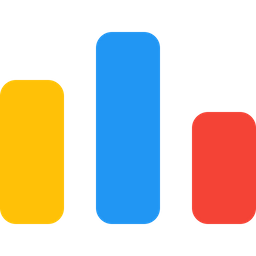
\includegraphics[scale=0.06]{cf.png} \ } 
            }}
            \\
            \textbf{B. Tech Computer Science and Engineering}
            \\
            {\textit{Minor in Mathematics}} 
            \\
            {Indian Institute of Technology, Madras} 
            \\
        \end{tabular}
    \end{minipage}\hfill
\end{table}
%%%%%%%%%%%%%%%%%%%%%%%%%%%%%%%%%%%%%%%%%%%%%%%%%%%%%%%%%%%%%%%%%%%%%%%%%%%%%%%%%%%%%%%%%%%%%%%%%%%%%%%%%%
\unskip
%%%%%%%%%%%%%%%%%%%%%%%%%%%%%%%%%%%%%%%%%%%%%%%%%%%%%%%%%%%%%%%%%%%%%%%%%%%%%%%%%%%%%%%%%%%%%%%%%%%%%%%%%%
\begin{multicols*}{2}
%%%%%%%%%%%%%%%%%%%%%%%%%%%%%%%%%%%%%%%%%%%%%%%%%%%%%%%%%%%%%%%%%%%%%%%%%%%%%%%%%%%%%%%%%%%%%%%%%%%%%%%%%%

\noindent
\resheading{\subheadingfont{EDUCATION}} 
\vspace{-0.1cm}
\\
\noindent
\projecttopic{B. Tech CSE \big \vert \hspace{3pt} CGPA 9.94} \hfill \mycal{Jul '21 - Present} 
\vspace{-0.1cm} \\
\projectdesc{Indian Institute of Technology Madras}  \hfill \myloc{Chennai, TN}
\vspace{-0.2cm} \\

\noindent
\projecttopic{HSC Class 12$^{\mathbf{th}}$ \big \vert \hspace{3pt} 98.17\%} \hfill \mycal{Apr '20 - Apr '21}
\vspace{-0.1cm} \\
\projectdesc{Pace Junior Science College}  \hfill \myloc{Mumbai, MH}
\vspace{-0.2cm} \\

\noindent
\projecttopic{ICSE Class 10$^{\mathbf{th}}$ \big \vert \hspace{3pt} 98.80\%} \hfill \mycal{Apr '18 - Apr '19}
\vspace{-0.1cm} \\
\projectdesc{Lilavatibai Podar High School} \hfill \myloc{Mumbai, MH}
\vspace{-0.2cm} \\

%%%%%%%%%%%%%%%%%%%%%%%%%%%%%%%%%%%%%%%%%%%%%%%%%%%%%%%%%%%%%%%%%%%%%%%%%%%%%%%%%%%%%%%%%%%%%%%%%%%%%%%%%%
\noindent
\resheading{\subheadingfont{EXPERIENCE}} \\ [0.1cm]

\noindent
\hrulefill \\ [-0.5cm]
\projecttopic{Software Internship at Optiver Amsterdam} \hfill \mycal{May'24 - Jul'24} 
\begin{itemize}[leftmargin=\myMargin]
    \setlength \itemsep{-0.1em}
    \item Worked in the Quant Research \& Data Team of Optiver Delta1
    \item Added functionality to create TCP/IP filters from session configuration files for the Network Parser and optimised them for performance.
    \item Added functionality to convert timestamps across timezones, accounting for Daylight Saving Time changes 
    \item Analysed SQL queries and designed a new OneTick database with Schema to replace a saturated PostGres time series database.
\end{itemize}
\vspace{3pt}

\noindent
\hrulefill \\ [-0.5cm]
\projecttopic{Team Avishkar Hyperloop, C\textcolor{red}{FI}} \hfill \mycal{Oct '22 - Present} 
\begin{itemize}[leftmargin=\myMargin]
    \setlength \itemsep{-0.1em}
    \item Part of Embedded Software Team of the \textbf{Main Control Unit} and \\ \textbf{Navigation Unit} of our Hyperloop Pod. 
    \item Used \textbf{RTOS, threading} and communication protocols like MQTT, CAN, etc. to collect and store data from over 20 sensors at \textbf{low latency}, \textbf{handling errors} appropriately.
    % \item Used communication protocols like MQTT, CAN, etc to collect data and send data to the base station/on-Pod Storage.
    \item Participated in the prestigious \textbf{European Hyperloop Week - Scotland 2023}, 
    among over 25 teams globally to represent the country.
\end{itemize}
\vspace{3pt}

\noindent
\hrulefill \\ [-0.5cm]
\projecttopic{Undergraduate Research - WiFi Sensing for IoT} \hfill  \mycal{Jan'24 - May'24}
\begin{itemize}[leftmargin=\myMargin]
    \setlength \itemsep{-0.1em}
    \item Created an end-to-end IoT pipeline for Human Activity Recognition using WiFi CSI (Channel State Information) Sensing
    \item Analysed the effect of compression on CSI data and its tradeoffs on the Network Bandwidth, Energy Consumption \& Sensing Accuracy.
    \item Submitted part of the work in AIoT workshop organised in Athens, Greece. 
\end{itemize}
\noindent
\projecttopic{Undergraduate Research - Custom Protocol Headers with P4 \\ for Network Application Support} \hfill \mycal{Ongoing}
\vspace{1pt}
\hrule 
\begin{itemize}[leftmargin=\myMargin]
    \setlength \itemsep{-0.1em}
    \item Ideation of a custom protocol header to improve network telemetry or security using P4 switch data plane programming language.
    \item Implementation with be done on Intel Tofino switches  
\end{itemize}
\vspace{3pt}

\noindent
\hrulefill \\ [-0.5cm]
\projecttopic{Tutor \& Contributor, \textcolor{nptel}{NPTEL}} \hfill \mycal{March '23 - Present}
\begin{itemize}[leftmargin=\myMargin]
    \setlength \itemsep{-0.1em}
    \item Created \textbf{YouTube tutorials} for previous years' GATE CS questions
    \item These tutorials aim to support applicants who may have limited access to resources
\end{itemize}

%%%%%%%%%%%%%%%%%%%%%%%%%%%%%%%%%%%%%%%%%%%%%%%%%%%%%%%%%%%%%%%%%%%%%%%%%%%%%%%%%%%%%%%%%%%%%%%%%%%%%%%%%%

 
\noindent
\resheading{\subheadingfont{SOFTWARE SKILLS}}
\vspace{-0.4cm}
 \begin{itemize}[leftmargin=\myMargin]
    \setlength \itemsep{-0.1em}
  \item \textbf{Languages}: C++, C, HDL (Verilog), OCaml, Python, Java, Prolog, SQL, x86, MIPS and 8085 ASM, HTML \& CSS, R 
  \item \textbf{Tools}: TI CCS, Git, \textbf{\LaTeX}, AutoCAD, GDB
\item \textbf{Libraries}: TI RTOS, NumPy, PyLops, Matplotlib
\vspace{-0.2cm}
  \end{itemize}
  

%%%%%%%%%%%%%%%%%%%%%%%%%%%%%%%%%%%%%%%%%%%%%%%%%%%%%%%%%%%%%%%%%%%%%%%%%%%%%%%%%%%%%%%%%%%%%%%%%%%%%%%%%%
\vspace{-0.1cm}
\noindent
\resheading{\subheadingfont{EXTRACURRICULAR ACTIVITIES}}
\begin{itemize}[leftmargin=\myMargin]
    \setlength \itemsep{-0.1em}
\item \textbf{Sports:} 
    Awarded 13 medals in various Track \& Field events and Best Athlete U14 in High School, Taekwondo Red Dan II Belt, NSO Athlete at IITM
\item Mentored freshmen, personally and academically, under \textbf{Saathi, IIT Madras}
\end{itemize}

%%%%%%%%%%%%%%%%%%%%%%%%%%%%%%%%%%%%%%%%%%%%%%%%%%%%%%%%%%%%%%%%%%%%%%%%%%%%%%%%%%%%%%%%%%%%%%%%%%%%%%%%%%

%%%%%%%%%%%%%%%%%%%%%%%%%%%%%%%%%%%%%%%%%%%%%%%%%%%%%%%%%%%%%%%%%%%%%%%%%%%%%%%%%%%%%%%%%%%%%%%%%%%%%%%%%%
%%%%%%%%%%%%%%%%%%%%%%%%%%%%%%%%%%%%%%%%%%%%%%%%%%%%%%%%%%%%%%%%%%%%%%%%%%%%%%%%%%%%%%%%%%%%%%%%%%%%%%%%%%
\columnbreak
%%%%%%%%%%%%%%%%%%%%%%%%%%%%%%%%%%%%%%%%%%%%%%%%%%%%%%%%%%%%%%%%%%%%%%%%%%%%%%%%%%%%%%%%%%%%%%%%%%%%%%%%%%

\noindent
\resheading{\subheadingfont{SCHOLASTIC ACHIEVEMENTS}}
\begin{itemize}[leftmargin=\myMargin]
\setlength \itemsep{-0.1em}
\item Awarded Sri V Ramachandran Prize for \textbf{Highest CGPA} in Semesters 3 \& 4 of B.Tech and Dual Degree in Computer Science 
\item Secured \textbf{AIR 5} in JEE Mains '19 out of 1 million students  %\hfill {[20XX]}%
\item Secured \textbf{AIR 161} in JEE Advanced '19\hfill
\item Secured \textbf{AIR 10} in Indian Statistical Institute Exam
\item Secured \textbf{AIR 21} in INChO and attended Orientation Camp for \\ International Chemistry Olympiad
\item Awarded KVPY Fellowship '21 with \textbf{AIR 338}
\item Winner of Mimamsa '22 at IISER Pune $\vert$ 4$^{th}$ place in Chemenigma '22 at IISC Bangalore $\vert$ Won Silver Medal in Homi Bhabha Science Competition (conducted in Maharashtra)
\end{itemize} 

%%%%%%%%%%%%%%%%%%%%%%%%%%%%%%%%%%%%%%%%%%%%%%%%%%%%%%%%%%%%%%%%%%%%%%%%%%%%%%%%%%%%%%%%%%%%%%%%%%%%%%%%%%
%\noindent
%\resheading{\subheadingfont{CODING ACHIEVEMENTS}}
% \begin{itemize}[ leftmargin=\myMargin]
%    \setlength \itemsep{-0.1em}
%  \item Rating 1806 \textcolor{blue}{Expert} on Codeforces
%%   \item Maximum Rating 1653 \textcolor{blue}{(3 
\includegraphics[scale=0.03]{bluestar.png})} on CodeChef
%  \item \textbf{ICPC 2022} - \textbf{AIR 151} and \textbf{Institute Rank 7} in Kanpur-Mathura Qualifier Round
%\item \textbf{AIR 3} in Shaastra CP Potpourri (Mixed-bag coding contest) \\ \small {\textit{[Shaastra is Asia's largest student-run Techfest]}} 
%    \item \normalsize{ \textbf{Global Rank 9} in CodeChef Starters 96} 
%    \item \normalsize{ \textbf{Global Rank 231} in Codeforces Round 881} 
%    \item \normalsize{ \textbf{Global Rank 373} in Google Farewell Round B} 
%    \item  \normalsize {1st place in Inter-School Java Competition in Mumbai}
%  \end{itemize}

%%%%%%%%%%%%%%%%%%%%%%%%%%%%%%%%%%%%%%%%%%%%%%%%%%%%%%%%%%%%%%%%%%%%%%%%%%%%%%%%%%%%%%%%%%%%%%%%%%%%%%%%%%
    
\noindent
\resheading{\subheadingfont{PROJECTS} }\\[0.1cm]

\noindent
\hrulefill \\ [-0.5cm]
\projecttopic{Java Compiler Design }
\mylink{insert link here}
\hfill    \textcolor{projDescColor}{\textit{Java, C}}  \\[0.1cm]
\projectdesc{CS3300 Course Project - Prof. Krishna Nandivada} \hfill \mycal{Jan-May '23} \\
\noindent
\vspace{-0.5cm}
\begin{itemize}[leftmargin=\myMargin]
    \item Implemented a MIPS compiler for a subset of Java with Lexical Analyser, Parsing, Type Checking, IR Generation, Register Allocation, Stack Handling, and MIPS code generation
\end{itemize}
\vspace{5pt}

\noindent
\hrulefill \\ [-0.5cm]
\projecttopic{OS Scheduler and Memory Management Unit Design}
\mylink{insert link here}
\hfill    \textcolor{projDescColor}{\textit{Java}}  \\[0.1cm]
\projectdesc{CS3500 Course Project - Prof. Prashant LA} \hfill \mycal{Jan-May '23} \\
\noindent
\vspace{-0.5cm}
\begin{itemize}[leftmargin=\myMargin]
    \setlength \itemsep{-0.1em}
    \item Implemented a Memory Management Unit with LRU Page replacement Policy
    \item Implemented a Multi-Level Feedback Queue Scheduler for processes
\end{itemize}
\vspace{5pt}

\noindent
\hrulefill \\ [-0.5cm]
\projecttopic{CPU Design} \mylink{https://github.com/Snehadeep-Gayen/Computer-Organisation-and-Architecture-Lab} 
\mylink{https://github.com/Snehadeep-Gayen/Simple_CPU_Design} 
\hfill    \textcolor{projDescColor}{\textit{Verilog}}  \\[0.1cm]
\projectdesc{CS2610 Course Project - Prof. C. Chandra Sekhar} \hfill \mycal{Jan-May '23} \\
\projectdesc{CS2310 Course Project - Prof. Ayon Chakraborty} \hfill \mycal{Jul-Nov '22}
\noindent
\vspace{-0.2cm}
\begin{itemize}[leftmargin=\myMargin]
    \setlength \itemsep{-0.1em}
    \item Implemented a CPU with \textbf{Register file} and \textbf{ALU} with instructions to perform Arithmetic 
    and Logical operations on both 8-bit integers and  12-bit floating-point numbers
    \item Built a combinational 8-bit CPU with structural gate-level Verilog 
\end{itemize}
\vspace{5pt}

\noindent
\hrulefill \\ [-0.5cm]
\projecttopic{Closeness Centrality Algorithm} \mylink{https://github.com/Snehadeep-Gayen/CENDY-Incremental-CC}
 \hfill \textcolor{projDescColor}{\textit{C++}} \\ [0.1cm]
\projectdesc{Project under Prof. Manikandan Narayanan} \hfill \mycal{May-Jun '23}
\vspace{-0.2cm}
\begin{itemize}[leftmargin=\myMargin]
    \item Implemented the CENDY algorithm, an on-line algorithm for updating Average Path Length and Closeness Centrality in a Dynamic Graph, based on this paper. \ \mylink{https://ieeexplore.ieee.org/stamp/stamp.jsp?tp=&arnumber=6729571&isnumber=6729471}
 \end{itemize}
\vspace{-0.2cm}

%%%%%%%%%%%%%%%%%%%%%%%%%%%%%%%%%%%%%%%%%%%%%%%%%%%%%%%%%%%%%%%%%%%%%%%%%%%%%%%%%%%%%%%%%%%%%%%%%%%%%%%%%%



%%%%%%%%%%%%%%%%%%%%%%%%%%%%%%%%%%%%%%%%%%%%%%%%%%%%%%%%%%%%%%%%%%%%%%%%%%%%%%%%%%%%%%%%%%%%%%%%%%%%%%%%%%


\noindent
\resheading{\subheadingfont{COURSES \& LABS}}
\small
\textbf{Computer Science}
\vspace{-0.3cm}
\begin{multicols}{2} 
    \scriptsize
\begin{itemize}[ leftmargin=\myMargin]
    \setlength \itemsep{-0.2em}
    \item Hi
    \columnbreak
    \item Hi
\end{itemize}
\end{multicols}
\noindent
\textbf{Mathematics}
\vspace{-0.3cm}
\begin{multicols}{2} 
    \scriptsize
\begin{itemize}[ leftmargin=\myMargin]
    \setlength \itemsep{-0.2em}
    \item Hi
    \columnbreak
    \item Hi
\end{itemize}
\end{multicols}
\noindent
\textbf{Economics}
\vspace{-0.3cm}
\begin{multicols}{2} 
    \scriptsize
\begin{itemize}[ leftmargin=\myMargin]
    \setlength \itemsep{-0.2em}
    \item Hi
    \columnbreak
    \item Hi
\end{itemize}
\end{multicols}

%%%%%%%%%%%%%%%%%%%%%%%%%%%%%%%%%%%%%%%%%%%%%%%%%%%%%%%%%%%%%%%%%%%%%%%%%%%%%%%%%%%%%%%%%%%%%%%%%%%%%%%%%%

\end{multicols*}
\end{document}